\section{3D Geometry}
\label{sec:3d_geometry}

\subsection{Lines in 3D}
\begin{frame}
    \frametitle{3D coordinates}
    \begin{figure}
        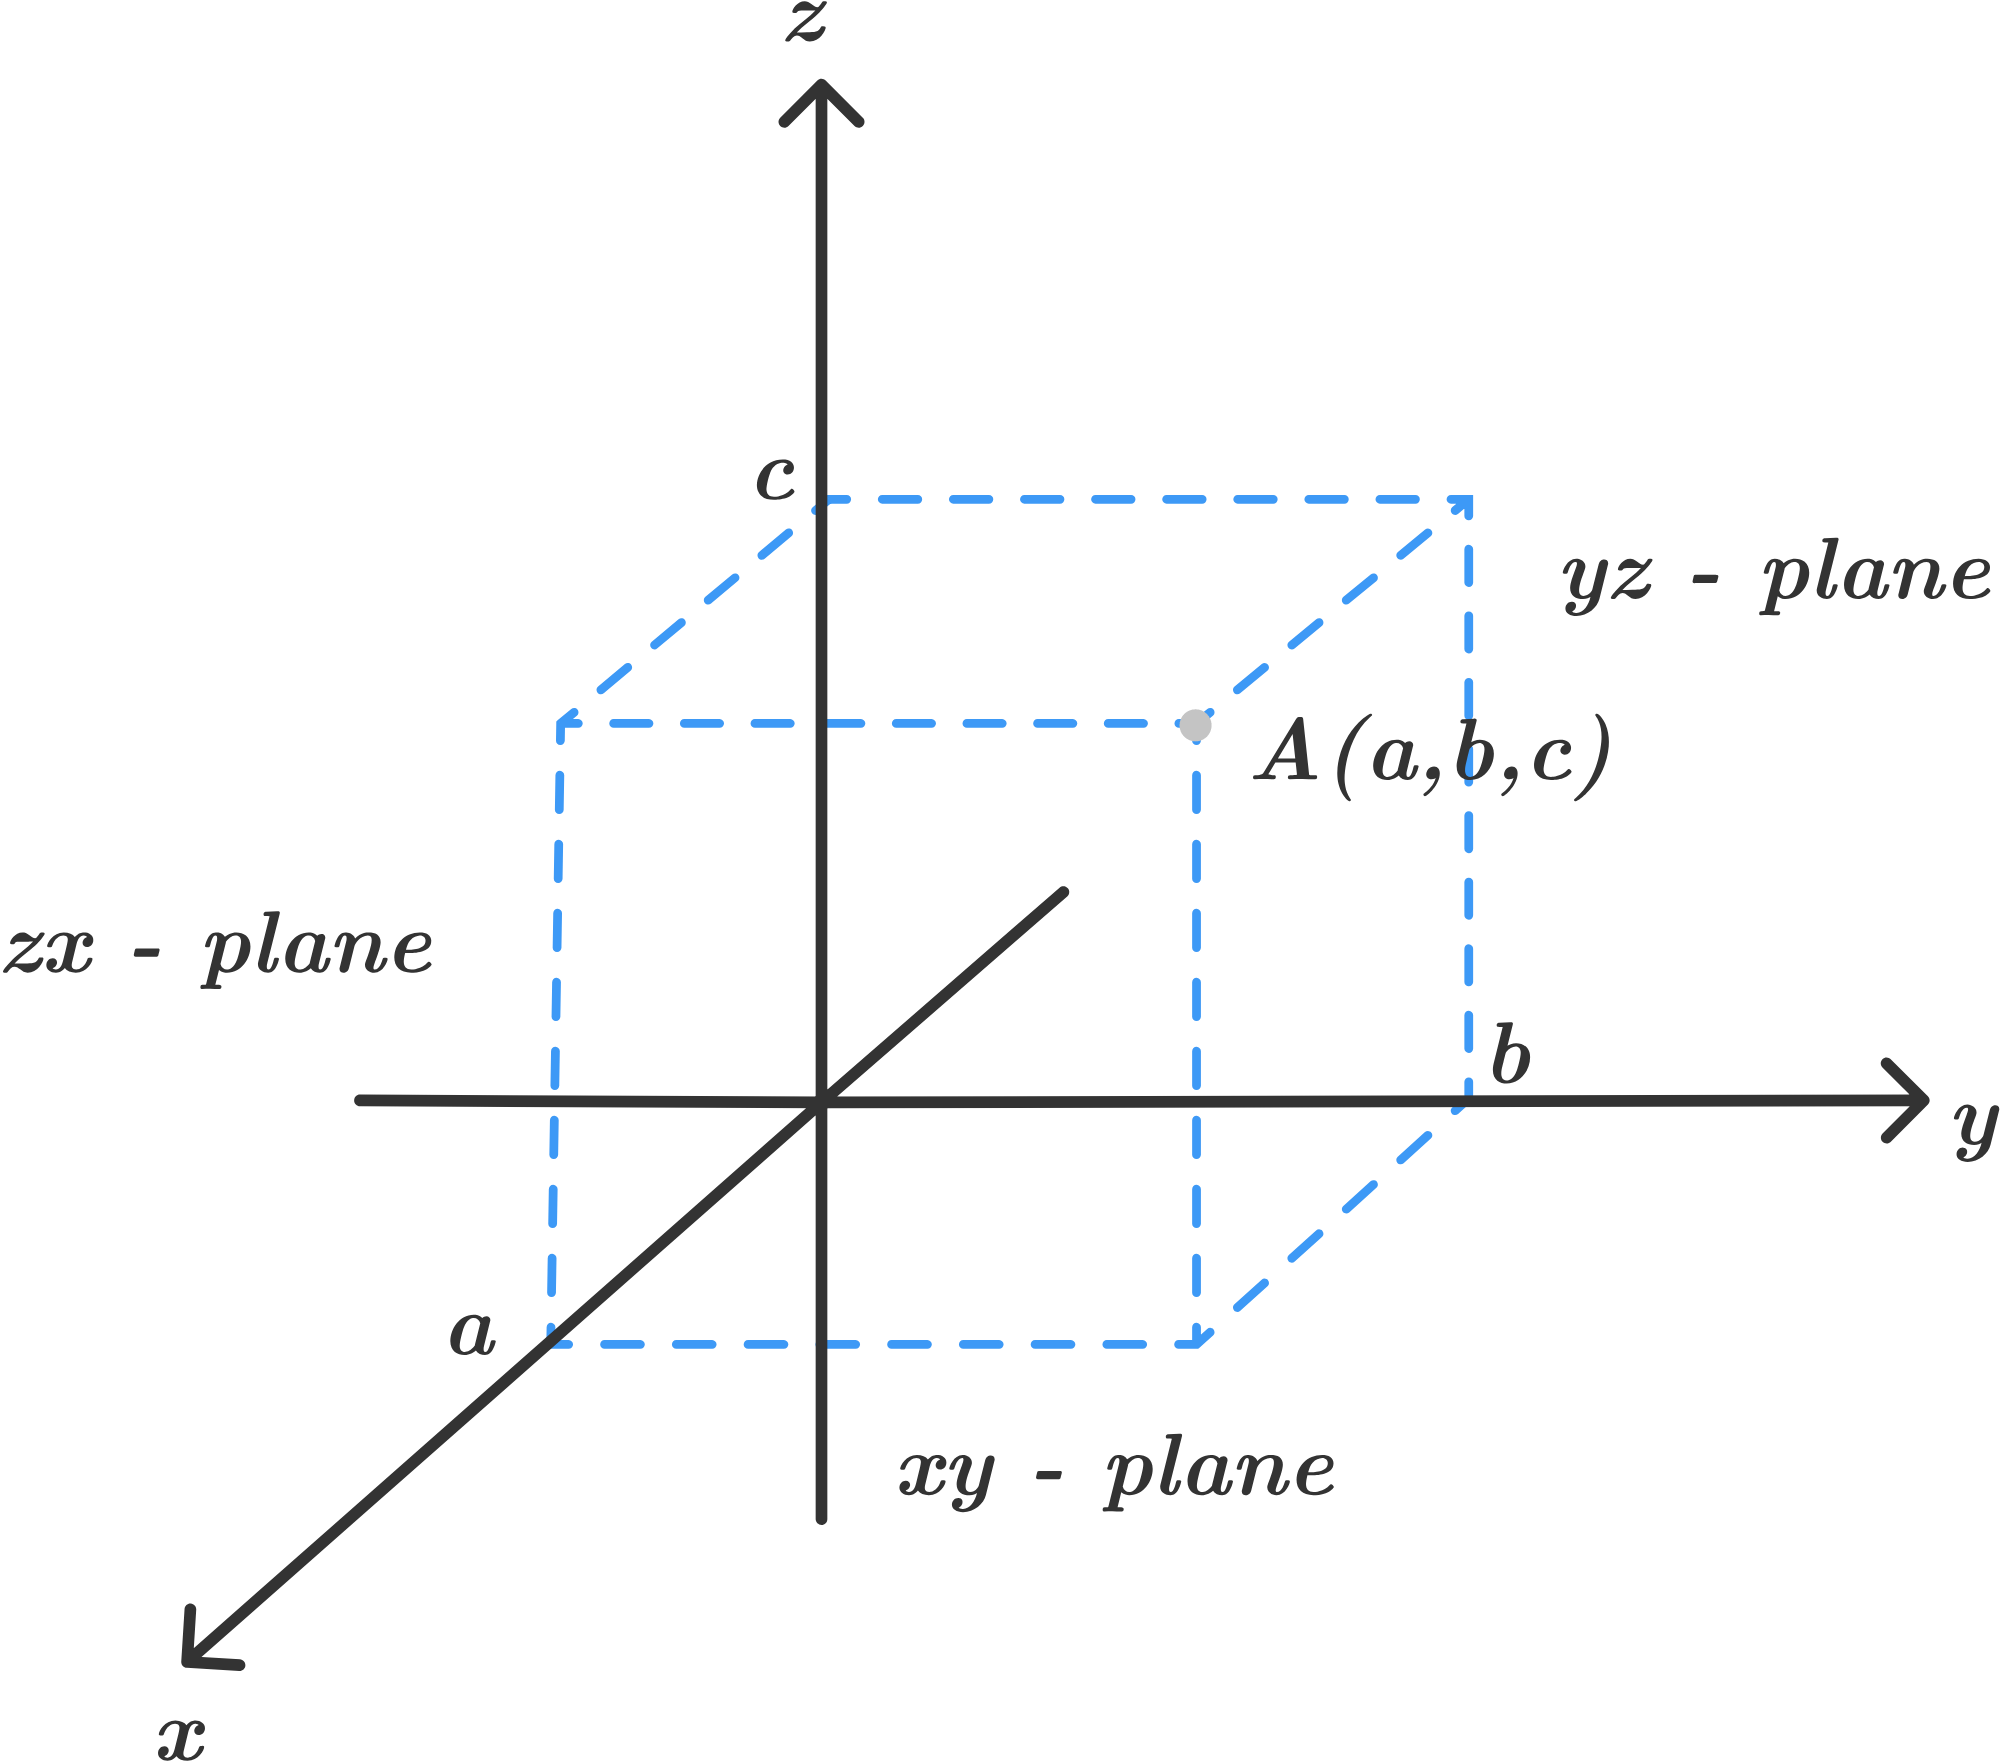
\includegraphics[scale=0.1]{3d_geometry/co_ordinate_plane.png}
        \caption{3D Coordinate Plane}
    \end{figure}
\end{frame}

\begin{frame}
    \frametitle{3D Coordinate System}
    \begin{itemize}
        \item The 3D coordinate system is defined by three mutually perpendicular axes: the x-axis, y-axis, and z-axis.
        \item A point in 3D space is represented by its coordinates \(P(x, y, z)\).
        \item The position vector of a point \(P\) in 3D space is given by:
        \[
        \vec{OP} = x\hat{\imath} + y\hat{\jmath} + z\hat{k}
        \]
    \end{itemize}       
\end{frame}

\begin{frame}
    \frametitle{Shifting the Origin}
    \begin{block}{Translation of Axes}
        Shifting the origin  to another point without changing the direction of axes is called \textbf{translation}.
    \end{block}
   Let the origin \(O\) be shifted to a new point \(O'\) with coordinates \(O'(x_0, y_0, z_0)\). The position vector of a point \(P(x,y,z)\) with respect to the new origin \(O'\) given by :
    \[
        \vec{O'P} = (x - x_0)\hat{\imath} + (y - y_0)\hat{\jmath} + (z - z_0)\hat{k}
    \]
\end{frame}

\begin{frame}
\frametitle{Distance Formula in 3D}
\begin{figure}
    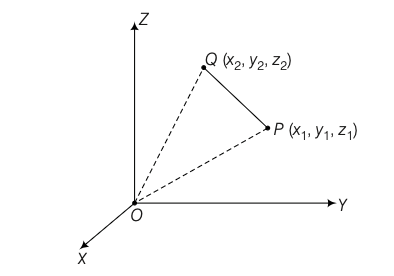
\includegraphics[scale=0.1]{3d_geometry/distance.png}
    \caption{Distance Formula in 3D}
\end{figure}
Let \(OP = x \hat{\imath} + y \hat{\jmath} + z \hat{k}\)  and \(OQ = x' \hat{\imath} + y' \hat{\jmath} + z' \hat{k}\) be two points in 3D space. The distance \(d\) between points \(P\) and \(Q\) is given by the formula:
\begin{align*}
    \vec{OQ} &= \vec{OP} + \vec{PQ} \\
    \vec{PQ} &= \vec{OQ} - \vec{OP} \\
    d &= |\vec{PQ}| = \sqrt{(x' - x)^2 + (y' - y)^2 + (z' - z)^2}
\end{align*}
\end{frame}

\begin{frame}
    \frametitle{Section Formula}
    \begin{figure}
        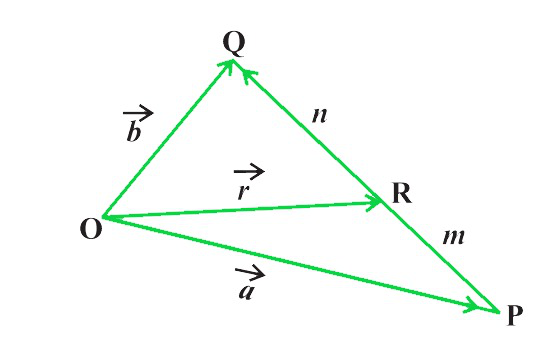
\includegraphics[scale=0.3]{3d_geometry/section.png}
        \caption{Section Formula in 2D}
    \end{figure} 
\end{frame}


\begin{frame}
    \begin{block}{Section Formula in 3D}
    Let \(P(x_1, y_1, z_1)\) and \(Q(x_2, y_2, z_2)\) be two points in 3D space with position vectors \( \vec{\mathbf{r}_1} \), \( \vec{\mathbf{r}_2} \) respectively. If a point \(R\) divides the line segment \(PQ\) in the ratio \(m:n\), then the position vector of point \(R\) is given by:
    \[
    \vec{\mathbf{r}} = \frac{m\vec{\mathbf{r}_2} + n\vec{\mathbf{r}_1}}{m+n}
    \]
    \end{block}
\end{frame}

\begin{frame}
    \frametitle{Proof of Section Formula}
    \begin{block}{Given}
    Point \(R\) divides line segment \(PQ\) internally in the ratio \(m:n\), where \(P\) and \(Q\) have position vectors \(\vec{\mathbf{a}}\) and \(\vec{\mathbf{b}}\) respectively.
    \end{block}
    
    \begin{block}{To Prove}
    The position vector of \(R\) is \(\vec{\mathbf{r}} = \frac{m\vec{\mathbf{b}} + n\vec{\mathbf{a}}}{m+n}\)
    \end{block}
    
    \begin{block}{Proof}
    Since \(R\) divides \(PQ\) in ratio \(m:n\):
    \begin{align}
        \frac{|\vec{PR}|}{|\vec{RQ}|} &= \frac{m}{n} \\
        \text{Since } \vec{PR} \text{ and } \vec{RQ} \text{ are collinear:} \quad \vec{PR} &= \frac{m}{n}\vec{RQ}
    \end{align}
    \end{block}
\end{frame}

\begin{frame}
    \frametitle{Proof of Section Formula (continued)}
    
    From vector addition: \(\vec{PR} + \vec{RQ} = \vec{PQ}\)
    
    Substituting \(\vec{PR} = \frac{m}{n}\vec{RQ}\):
    \begin{align}
        \frac{m}{n}\vec{RQ} + \vec{RQ} &= \vec{PQ} \\
        \vec{RQ}\left(\frac{m}{n} + 1\right) &= \vec{PQ} \\
        \vec{RQ} &= \frac{n}{m+n}\vec{PQ}
    \end{align}

\end{frame}


\begin{frame}
 
    Since \(\vec{PQ} = \vec{\mathbf{b}} - \vec{\mathbf{a}}\) and \(\vec{RQ} = \vec{\mathbf{b}} - \vec{\mathbf{r}}\):
    \begin{align}
        \vec{\mathbf{b}} - \vec{\mathbf{r}} &= \frac{n}{m+n}(\vec{\mathbf{b}} - \vec{\mathbf{a}}) \\
        \vec{\mathbf{r}} &= \vec{\mathbf{b}} - \frac{n}{m+n}(\vec{\mathbf{b}} - \vec{\mathbf{a}}) \\
        \vec{\mathbf{r}} &= \frac{m\vec{\mathbf{b}} + n\vec{\mathbf{a}}}{m+n}
    \end{align}
  
\end{frame}

\begin{frame}
\frametitle{Direction Ratios}
    The direction ratios of a line are any three numbers that are proportional to the direction cosines of the line. If a line has direction cosines \(l, m, n\), then its direction ratios can be represented as \(a, b, c\) such that:
    \begin{align*}
        l &= \frac{a}{\sqrt{a^2 + b^2 + c^2}} =  k a \\
        m &= \frac{b}{\sqrt{a^2 + b^2 + c^2}}  = k b \\
        n &= \frac{c}{\sqrt{a^2 + b^2 + c^2}} = k c
    \end{align*}
\begin{itemize}
    \item It is evident that the direction ratios are not unique, as they can be scaled by any non-zero constant \(k\).
    \item However, the ratios \(a:b:c\) remain constant regardless of the scaling
\end{itemize}
\end{frame}

\begin{frame}
    \frametitle{Direction Cosines vs. Direction Ratios: The Intuition}
    \begin{itemize}
        \item \textbf{Direction Cosines (DCs):} A unique, standardized recipe. They tell you how much to travel along each axis to move exactly one unit along the line. The sum of their squares is always 1: \(l^2 + m^2 + n^2 = 1\).
        \item \textbf{Direction Ratios (DRs):} A flexible, proportional recipe. They tell you the ratio of movement along the axes. For every 'a' units in x, you move 'b' units in y and 'c' units in z. They are not unique; any scalar multiple represents the same direction.
    \end{itemize}
\end{frame}

\begin{frame}
    \frametitle{Direction Cosines (DCs): Mathematical Definition}
    Let a vector \(\vec{v}\) make angles \(\alpha, \beta, \gamma\) with the positive X, Y, and Z axes.
    \begin{itemize}
        \item \(l = \cos(\alpha)\)
        \item \(m = \cos(\beta)\)
        \item \(n = \cos(\gamma)\)
    \end{itemize}

    For a vector \(\vec{v} = (x, y, z)\) with magnitude \(|\vec{v}| = \sqrt{x^2 + y^2 + z^2}\):
    \[ l = \frac{x}{|\vec{v}|}, \quad m = \frac{y}{|\vec{v}|}, \quad n = \frac{z}{|\vec{v}|} \]
    A key property is that \(l^2 + m^2 + n^2 = 1\).
\end{frame}

\begin{frame}
    \frametitle{Converting Direction Ratios to Direction Cosines}
    If you have direction ratios \((a, b, c)\), you can find the direction cosines \((l, m, n)\) by normalizing them:
    \[ l = \frac{a}{\sqrt{a^2 + b^2 + c^2}} \]
    \[ m = \frac{b}{\sqrt{a^2 + b^2 + c^2}} \]
    \[ n = \frac{c}{\sqrt{a^2 + b^2 + c^2}} \]
    This process creates a unit vector, which is what the direction cosines represent.
\end{frame}


\begin{frame}
    \frametitle{Equation of a Line passing through a given point and parallel to a given vector}
    \begin{figure}
        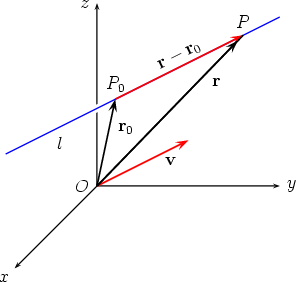
\includegraphics[scale=0.4]{3d_geometry/line_parallel_vector.png}
        \caption{Line in 3D space}
    \end{figure}
\end{frame}


\begin{frame}
\frametitle{Equation of a Line passing through a given point and parallel to a given vector}
    Let \(P_{0}(x_0, y_0, z_0)\) be a point on the line and \(P_{1}(x_1, y_1, z_1)\) be another point on the line. The direction vector of the line can be defined as \(\vec{P_{0}P_{1}} = \vec{r}_1 - \vec{r}_0\), where \(\vec{r}_0\) and \(\vec{r}_1\) are the position vectors of \(P_0\) and \(P_1\) respectively. The vector equation of the line can be expressed as:
    \[
    \vec{r} - \vec{r_0} = t\vec{v}
    \]
    where \(t\) is a scalar parameter. 
\end{frame}
\begin{frame}
    \frametitle{Equation of a Line: Two-Point Form}
    Given two points on the line, \(A(x_1, y_1, z_1)\) and \(B(x_2, y_2, z_2)\).
    \begin{block}{Vector Form}
        Let the position vectors of A and B be \(\vec{a}\) and \(\vec{b}\). The direction vector is \(\vec{d} = \vec{b} - \vec{a}\). The equation of the line is:
        \[ \vec{r} = \vec{a} + \lambda(\vec{b} - \vec{a}) \]
    \end{block}
    \begin{block}{Cartesian Form}
        The direction ratios are \((x_2 - x_1, y_2 - y_1, z_2 - z_1)\). The equation is:
        \[ \frac{x - x_1}{x_2 - x_1} = \frac{y - y_1}{y_2 - y_1} = \frac{z - z_1}{z_2 - z_1} \]
    \end{block}
\end{frame}

\begin{frame}
    \frametitle{Equation of a Line: Symmetric Form}
    If the direction ratios of the line are \(a, b, c\) and it passes through point \(P_0(x_0, y_0, z_0)\), the symmetric form of the line's equation is:
    \[
    \frac{x - x_0}{a} = \frac{y - y_0}{b} = \frac{z - z_0}{c}
    \]
    This form is particularly useful when the direction ratios are known.
\end{frame}

\begin{frame}
    \frametitle{Angle between Two Lines}
    To find the angle \(\theta\) between two lines with direction ratios \((a_1, b_1, c_1)\) and \((a_2, b_2, c_2)\), we use the formula:
    \[
    \cos(\theta) = \frac{a_1 a_2 + b_1 b_2 + c_1 c_2}{\sqrt{a_1^2 + b_1^2 + c_1^2} \sqrt{a_2^2 + b_2^2 + c_2^2}}
    \]
    This formula is derived from the dot product of the direction vectors.
\end{frame}

\begin{frame}
    \frametitle{Angle between Two Lines}
    Let \(\vec{r} = \vec{a+ \lambda b}\) and \(\vec{r'} = vec{a'} + \alpha b'\) be two straight line in 3D space. The angle \(\theta\) between the two lines is given by:
    \[
    \cos(\theta) = \frac{\vec{b} \cdot \vec{b'}}{|\vec{b}| |\vec{b'}|}
    \]
    where \(\vec{b}\) and \(\vec{b'}\) are the direction vectors of the lines.

    This is because the angle between the two lines is equal to the angle between their direction vectors.
\end{frame}

\begin{frame}
    \frametitle{Perpendicular Distance from a Point to a Line in 3D}
    To find the perpendicular distance \(d\) from a point \(P_0(x_0, y_0, z_0)\) to a line defined by a point \(P_1(x_1, y_1, z_1)\) and direction vector \(\vec{v} = (a, b, c)\), we use the formula:
    \[
    d = \frac{|\vec{P_0P_1} \times \vec{v}|}{|\vec{v}|}
    \]
    where \(\vec{P_0P_1} = (x_1 - x_0, y_1 - y_0, z_1 - z_0)\) is the vector from the point to the line.        
\end{frame}


\begin{frame}
\begin{figure}
    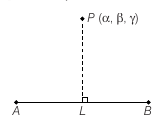
\includegraphics[scale=0.9]{3d_geometry/perpendicular_line.png}
    \caption{Perpendicular Distance from a Point to a Line in 3D}
\end{figure}
\end{frame}
\begin{frame}
    \frametitle{Perpendicular Distance from a Point to a Line in 3D}
    Let the line AB is defined by 
    \[\frac{x-x_{1}}{a} = \frac{y-y_{1}}{b} = \frac{z-z_{1}}{c}\]
    and \(P(\alpha, \beta, \gamma)\) be the point. The perpendicular distance \(d\) from point \(P\) . The co-ordinates of the point \(L\) can be identified as:
    \[L(x_{1}+at, y_{1}+bt, z_{1}+ct)\]  
    where \(t\) is a scalar.. The vector \(\vec(AL)\) is given by 
    \[\vec(AL) = (x_{1}+at - x_{1}, y_{1}+bt - y_{1}, z_{1}+ct - z_{1}) = (at, bt, ct)\] 
\end{frame} 

\begin{frame}
    
    vector \(\vec{PL} \) is given by 
    \[\vec{PL} = (x_{1}+at - \alpha, y_{1}+bt - \beta, z_{1}+ct - \gamma)\]  
    
    Since \(AL \perp PL\), we can equate following

    \[(x_{1}+at-\alpha)(a) + (y_{1}+bt-\beta)(b) + (z_{1}+ct-\gamma)(c) = 0\]

    This can be solved for \(t\) to find the point \(L\) on the line.

\end{frame}

\begin{frame}
    \frametitle{Shortest Distance between two skew straight lines in 3D}

    Let the two lines are given by :
    \begin{align*}
    l_{1} = a_{1} + \lambda b_{1} \\
    l_{2} = a_{2} + \mu b_{2}   
    \end{align*}
    where \(a_{1}\) and \(a_{2}\) are position vectors of points on the lines, and \(b_{1}\) and \(b_{2}\) are direction vectors of the lines. Let \(\vec{AB}\) be the line through points \(a_{1}\) and \(a_{2}\). The perpendicular to both the lines can be found by taking the cross product of their direction vectors, i.e., \(\vec{b_{1}} \times \vec{b_{2}}\). The shortest distance \(d\) between the two skew lines is given by the projection of the line segment \(\vec{AB}\) onto the direction of the unit perpendicular, which can be calculated using the formula:

    \begin{align*}
    d = \frac{|\vec{AB} \cdot (\vec{b_{1}} \times \vec{b_{2}})|}{|\vec{b_{1}} \times \vec{b_{2}}|}
    \end{align*}

\end{frame}



\subsection{Planes in 3D}

\begin{frame}
    \frametitle{What is a Plane?}
    A plane is a surface such that if any two points on it are joined by a straight line, then every point on that line lies on the surface.
    \begin{block}{General Form}
        The general equation of a plane in 3D space is given by:
        \[
        Ax + By + Cz + D = 0
        \]
        where \(A\), \(B\), \(C\), and \(D\) are constants, and \(A\), \(B\), and \(C\) are not all zero.
    \end{block}
\end{frame}

\begin{frame}
    \frametitle{Proof of the Plane Equation}
    Let \(P(x_{1},x_{2},x_{3}) \) and \(Q(x_{2},y_{2},z_{2})\) be two points on the plane. Then we can write 
    \[
    ax_{1} + by_{1} + cz_{1} + d = 0
    \]
    and
    \[
    ax_{2} + by_{2} + cz_{2} + d = 0
    \]

    Let \(R\) be any point on the line joining \(P\) and \(Q\) with a ratio \(\lambda : 1\). Then the coordinates of \(R\) can be expressed as: 

    \[R\left(\frac{x_{1} + \lambda x_{2}}{1+\lambda}, \frac{y_{1} + \lambda y_{2}}{1+\lambda}, \frac{z_{1} + \lambda z_{2}}{1+\lambda}\right)\]
\end{frame} 

\begin{frame}
   Since \(R\) lies on the plane, it must satisfy the plane equation:

   \[
   a\left(\frac{x_{1} + \lambda x_{2}}{1+\lambda}\right) + b\left(\frac{y_{1} + \lambda y_{2}}{1+\lambda}\right) + c\left(\frac{z_{1} + \lambda z_{2}}{1+\lambda}\right) + d = 0
   \]

   Multiplying through by \(1+\lambda\) gives:

   \[
   a(x_{1} + \lambda x_{2}) + b(y_{1} + \lambda y_{2}) + c(z_{1} + \lambda z_{2}) + d(1+\lambda) = 0
   \]
\end{frame} 

\begin{frame}
   Rearranging terms leads to:

   \[
   (ax_{1} + by_{1} + cz_{1} + d) + \lambda (ax_{2} + by_{2} + cz_{2} + d) = 0
   \]

   Since both terms must equal zero, we have:

   \[
   ax_{1} + by_{1} + cz_{1} + d = 0
   \]
   and
   \[
   ax_{2} + by_{2} + cz_{2} + d = 0
   \]

   Thus, the line joining \(P\) and \(Q\) lies entirely within the plane.

\end{frame}

\begin{frame}
    \frametitle{Equation of a Plane in Normal Form}
    \begin{figure}
        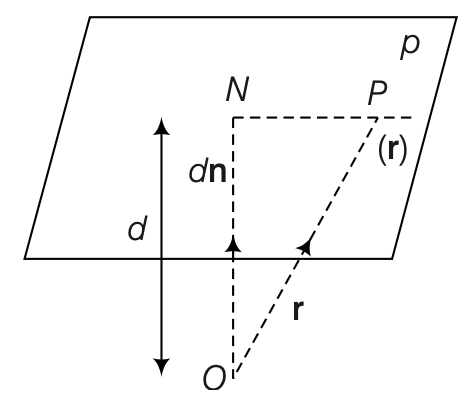
\includegraphics[scale=0.4]{3d_geometry/normal_form.png}
        \caption{Plane in 3D space}
    \end{figure}
\end{frame}

\begin{frame}
\frametitle{Equation of Plane in Normal Form}
    Let \(O\) be the origin and \(ON\) be the perpendicular from the origin \(O\) to the given plane \(\pi\) such that \(ON = d \hat{n}\), where \(\hat{n}\) is the unit normal vector to the plane where \( d\) is the perpendicular distance from the origin to the plane. 
    \begin{align*} 
        OP &= \vec{r} \\ 
        NP &\perp ON \\ 
        NP \cdot ON &= 0 \\ 
        (OP - ON) \cdot ON &= 0 \\
        ( \vec{r} - d \hat{n}) \cdot d\hat{n} &= 0 \\
        \vec{r} \cdot d \hat{n} - d^2 \hat{n} \cdot \hat{n} &= 0 \\
        \vec{r} \cdot \hat{n} &= d
    \end{align*}
\end{frame}

\begin{frame}
\frametitle{Normal form Cartesian Form}
 Let \(P(x,y,z)\) be a point on the plane and \( l,m,n\) be the direction cosines of the normal to the plane. The equation of the plane in Cartesian form is given by: 
 \begin{align*}
 r \cdot \hat{n} &= d \\
 x \hat{\imath} + y \hat{\jmath} + z \hat{k} \cdot l \hat{\imath} + m \hat{\jmath} + n \hat{k} &= d \\
 lx + my + nz &= d
 \end{align*}
where \(d\) is the perpendicular distance from the origin to the plane. 
\end{frame} 

\begin{frame}
\frametitle{Normal form vs General form of Plane Equation}
\begin{itemize}
\item The normal form  of the plane given by \( \vec{r} \cdot \hat{n} = d\) . In the cartesian form  
\[ lx + my + nz = d \] 
where \(l,m,n\) are the direction cosines of the normal to the plane as the normal is a unit vector.

\item The general form of the plane is given by \(Ax + By + Cz + D = 0\) where \(A,B,C\) are the direction ratios of the normal to the plane. The coefficents of \(A,B,C\) in the general form are the direction ratios of the normal to the plane.
\end{itemize}
\end{frame}

\begin{frame}
    \frametitle{Vector Equation of a Plane Passing Through
a Given Point and Normal to a Given Vector}

Let \( \vec{r} \) be the position vector of a point \( P(x,y,z) \) on the plane, and let \( \vec{a} \) be the position vector of a given point \( A(x_0,y_0,z_0) \) on the plane. The vector equation of the plane can be expressed as:

\[
(\vec{r} - \vec{a}) \cdot \hat{n} = 0
\]

where \( \hat{n} \) is the unit normal vector to the plane.

\end{frame} 

\begin{frame}
\frametitle{Equation of a Plane Passing Through
a Given Point and Parallel to Two
Given Vectors}
We can infer following observations :
\begin{enumerate}
    \item A vector on the plane is given by \( \vec{r} - \vec{a} \) where \(\vec{r},\vec{a}\) are the position vectors of points \(P\) and \(A\) respectively.
    \item As two vectors \( \vec{b} \) and \( \vec{c} \) are parallel to the plane, the vector \( \vec{r} - \vec{a} \) is coplanar with vectors \( \vec{b} \) and \( \vec{c} \). 
    \item This means \((\vec{r} - \vec{a}) = \lambda_1 \vec{b} + \lambda_2 \vec{c}\) for some scalars \(\lambda_1\) and \(\lambda_2\).
    \item That is \(\vec{r} = \vec{a} + \lambda_1 \vec{b} + \lambda_2 \vec{c}\)
\end{enumerate}     
\end{frame}